%!TEX root = *.tex
%%%%%%%%%%%%%%%%%%
% メモ
\begin{comment}

\end{comment}
% カウンタのリセット
\setcounter{eqNo}{0}
\setcounter{figure}{0}
% 解答
\noindent {\large【解答】\par}

\noindent (1)\,
$f=\dfrac{1}{T},\,\lambda =vT$.


\noindent (2)\,
位置\x における入射波は,波が原点から伝わるのにかかる時間$\dfrac{x}{v}$だけ原点の振動より遅れる.
よって,時刻$t$における位置\x での入射波の変位$y_1$は,
時刻$t-\dfrac{x}{v}$における原点の変位に等しい.
\begin{align*}
  y_1 = A \sin \frac{2\pi}{T}\left(t-\frac{x}{v}\right)
\end{align*}

\noindent (3)\,
反射波が原点から固定端を通り位置\x に伝わるまでに$2L-x$だけ移動するので,要する時間は$\frac{2L-x}{v}$である.

また,固定端反射によって位相は$\pi$だけずれる.

時刻$t$における位置\x での反射波の変位$y_2$は,
時刻$t-\frac{2L-x}{v}$における原点の変位を$\pi$だけ位相をずらしたもの.
\begin{align*}
  y_2 = A \sin \left(\frac{2\pi}{T}\left(t-\frac{2Lx}{v}\right)+\pi\right) = -A\sin\frac{2\pi}{T}\left(t-\frac{2Lx}{v}\right)
\end{align*}

\noindent (4)\,
(2),(3)より重ね合わせの理により,位置\x における媒質の変位は\y は
\begin{align*}
  y &= y_1+y_2 
  = A \sin \frac{2\pi}{T}\left(t-\frac{x}{v}\right)
  - A \sin \frac{2\pi}{T}\left(t-\frac{2Lx}{v}\right) \\
  &= 2A \cos\left(\frac{1}{2}\frac{2\pi}{T}\left(t-\frac{x}{v}+t-\frac{2L-x}{v}\right)\right)\sin\left(\frac{1}{2}\frac{2\pi}{T}\left(t-\frac{x}{v}-t+\frac{2L-x}{v}\right)\right) \\
  &= 2A\sin \frac{2\pi}{T}\left(\frac{L-x}{v}\right) \cos \frac{2\pi}{T}\left(t-\frac{L}{v}\right)
\end{align*}
となる.位置\x において,$2A\sin \frac{2\pi}{T}\left(\frac{L-x}{v}\right)$は時刻$t$によらないので,その位置における振幅を表し,
$\cos \frac{2\pi}{T}\left(t-\frac{L}{v}\right)$は時刻$t$にのみ依存した振動を表す.したがって,波形の進行しない定在波である.



{
\begin{wrapfigure}{r}{.4\columnwidth}
  \vspace{-\intextsep}
  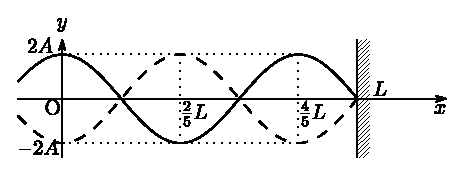
\includegraphics[width=.4\columnwidth]{../graphs/jumon_75_sol.eps}
\end{wrapfigure}
\noindent (5)\,
固定端は定在波の節となる.また,節と腹の間隔は$\frac{\lambda}{4}=\frac{L}{5}$.
(4)の結果から定在波の振幅の最大値は$2A$なので下図を得る.


\par}

\noindent
〔別解〕(4)の結果を用いる.\par 
定在波の振幅は$\cos \frac{2\pi}{T}\left(t-\frac{L}{v}\right)=\pm 1$のときに最大となる.このとき,
\begin{align*}
  y &= \pm 2A\sin \frac{2\pi}{T}\left(\frac{L-x}{v}\right) 
  = \pm 2A\sin 2\pi \frac{L-x}{\lambda} \\
  &= \pm 2A\sin \left(\frac{5}{2}\pi - \frac{5\pi x}{2L}\right) \\
  &= \pm 2A\cos\frac{5\pi}{2L}x
\end{align*}
\noindent
となり同様の結果が得られる.




%%%%%%%%%%%%%%%%%%%